\documentclass[12pt,aspectratio=169]{beamer}

% Input
\usepackage[utf8]{inputenc}
\usepackage[T1]{fontenc}
\usepackage[letterspace=100]{microtype}
\usepackage{upquote}

% Beamer
\usetheme{metropolis}
\usepackage[sfdefault]{FiraSans}
\usepackage{xcolor}
\definecolor{blue}{HTML}{002957}
\definecolor{red}{HTML}{F1563F}
\setbeamercolor{palette primary}{fg=white,bg=blue}
\setbeamercolor{title separator}{fg=red,bg=blue}
\setbeamercolor{frametitle}{fg=white,bg=blue}
\setbeamercolor{progress bar}{fg=red,bg=blue}
\setbeamercolor{alerted text}{fg=red,bg=blue}
\makeatletter
\setlength{\metropolis@titleseparator@linewidth}{2pt}
\setlength{\metropolis@progressonsectionpage@linewidth}{2pt}
\setlength{\metropolis@progressinheadfoot@linewidth}{2pt}
\makeatother

% Graphics
\usepackage{graphicx}
\usepackage{epstopdf}
\DeclareGraphicsExtensions{.png,.pdf,.eps}
\tikzset{
  invisible/.style={opacity=0},
  visible on/.style={alt={#1{}{invisible}}},
  alt/.code args={<#1>#2#3}{%
    \alt<#1>{\pgfkeysalso{#2}}{\pgfkeysalso{#3}} % \pgfkeysalso doesn't change the path
  },
}
\usetikzlibrary{arrows, shapes}

% Various
\usepackage{hyperref}
\usepackage{minted}
\usepackage{fontawesome}

% Title
\title{Plone and Volto in a Jamstack Project}
\subtitle{Plone Conference 2020}
\date{7.12.2020}
\author{Asko Soukka}
\institute{\vspace{-0.5cm}
\includegraphics[height=1.5cm]{images/jyu-vaaka-kaksikielinen.eps}\hfill
\includegraphics[width=0.20\paperwidth]{images/volto-logo.eps}\raisebox{0.075\paperwidth}{\fontsize{40}{40}\selectfont~+~}
\includegraphics[width=0.20\paperwidth]{images/Gatsby_Monogram.eps}}

\newcommand{\setmytemplate}{\usebackgroundtemplate{\begin{picture}(0,0)(-5,250)\footnotesize\href{https://twitter.com/datakurre}{\faTwitter~datakurre}\end{picture}\begin{picture}(0,0)(-330,298)
\includegraphics[width=0.40\paperwidth]{images/plone-icon.pdf}\end{picture}}}

\newcommand{\setalttemplate}{\usebackgroundtemplate{\begin{picture}(0,0)(-5,250)\footnotesize\href{https://twitter.com/datakurre}{\faTwitter~datakurre}\end{picture}\begin{picture}(0,0)(-260,278)
\includegraphics[width=0.40\paperwidth]{images/volto-logo.eps}\end{picture}}}

\begin{document}

% define tikz styles
\definecolor{gatsby}{HTML}{663399}
\tikzstyle{block} = [rectangle, fill=gatsby, text=white,
    text width=5em, text centered, rounded corners, minimum height=4em]
\tikzstyle{example} = [rectangle, draw, dashed,
    text width=5em, text centered, rounded corners, minimum height=4em]
\tikzstyle{line} = [draw, -latex']

\setbeamertemplate{background canvas}[default]
\maketitle

%---------------------------------------------------------------------------------------

\setbeamertemplate{background canvas}[default]
\begin{frame}{Backend: Plone \& Volto}
\begin{picture}(0,0)(29,128)
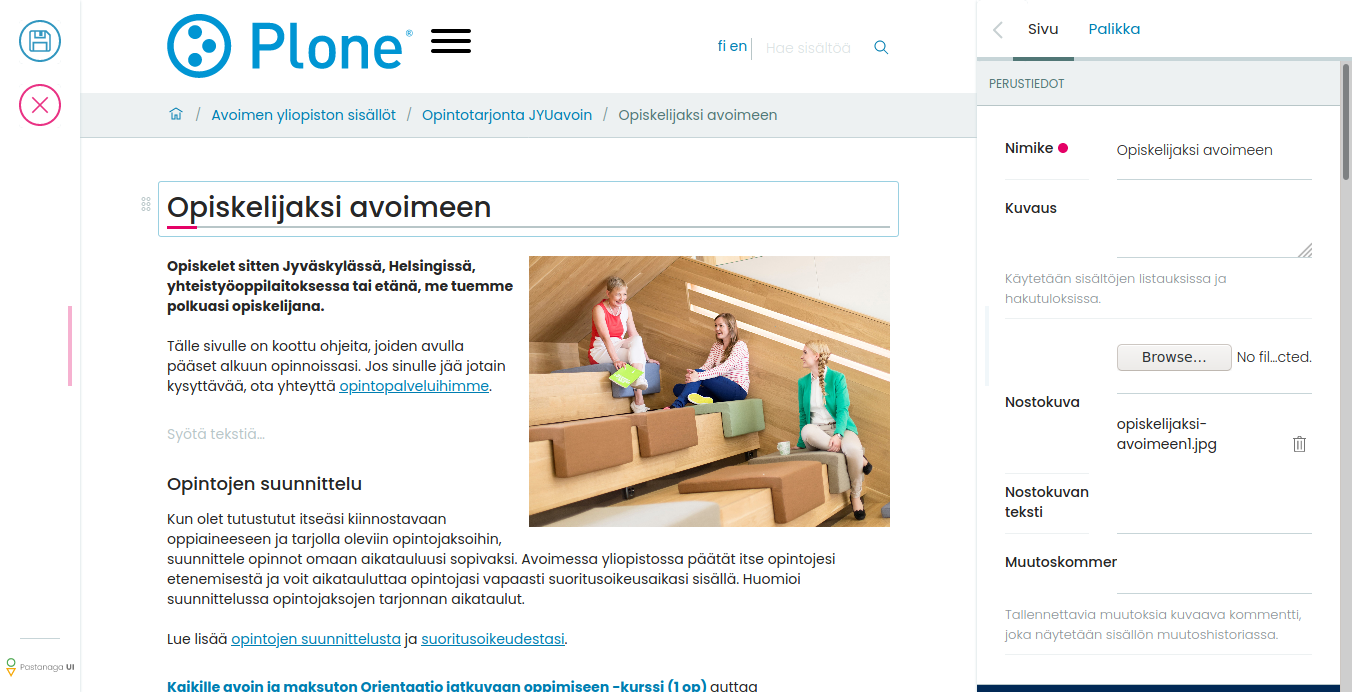
\includegraphics[width=1\paperwidth]{images/study-guide-03.png}
\end{picture}
\end{frame}

\setbeamertemplate{background canvas}[default]
\begin{frame}{Frontend: GatsbyJS Jamstack}
\begin{picture}(0,0)(29,562.5)
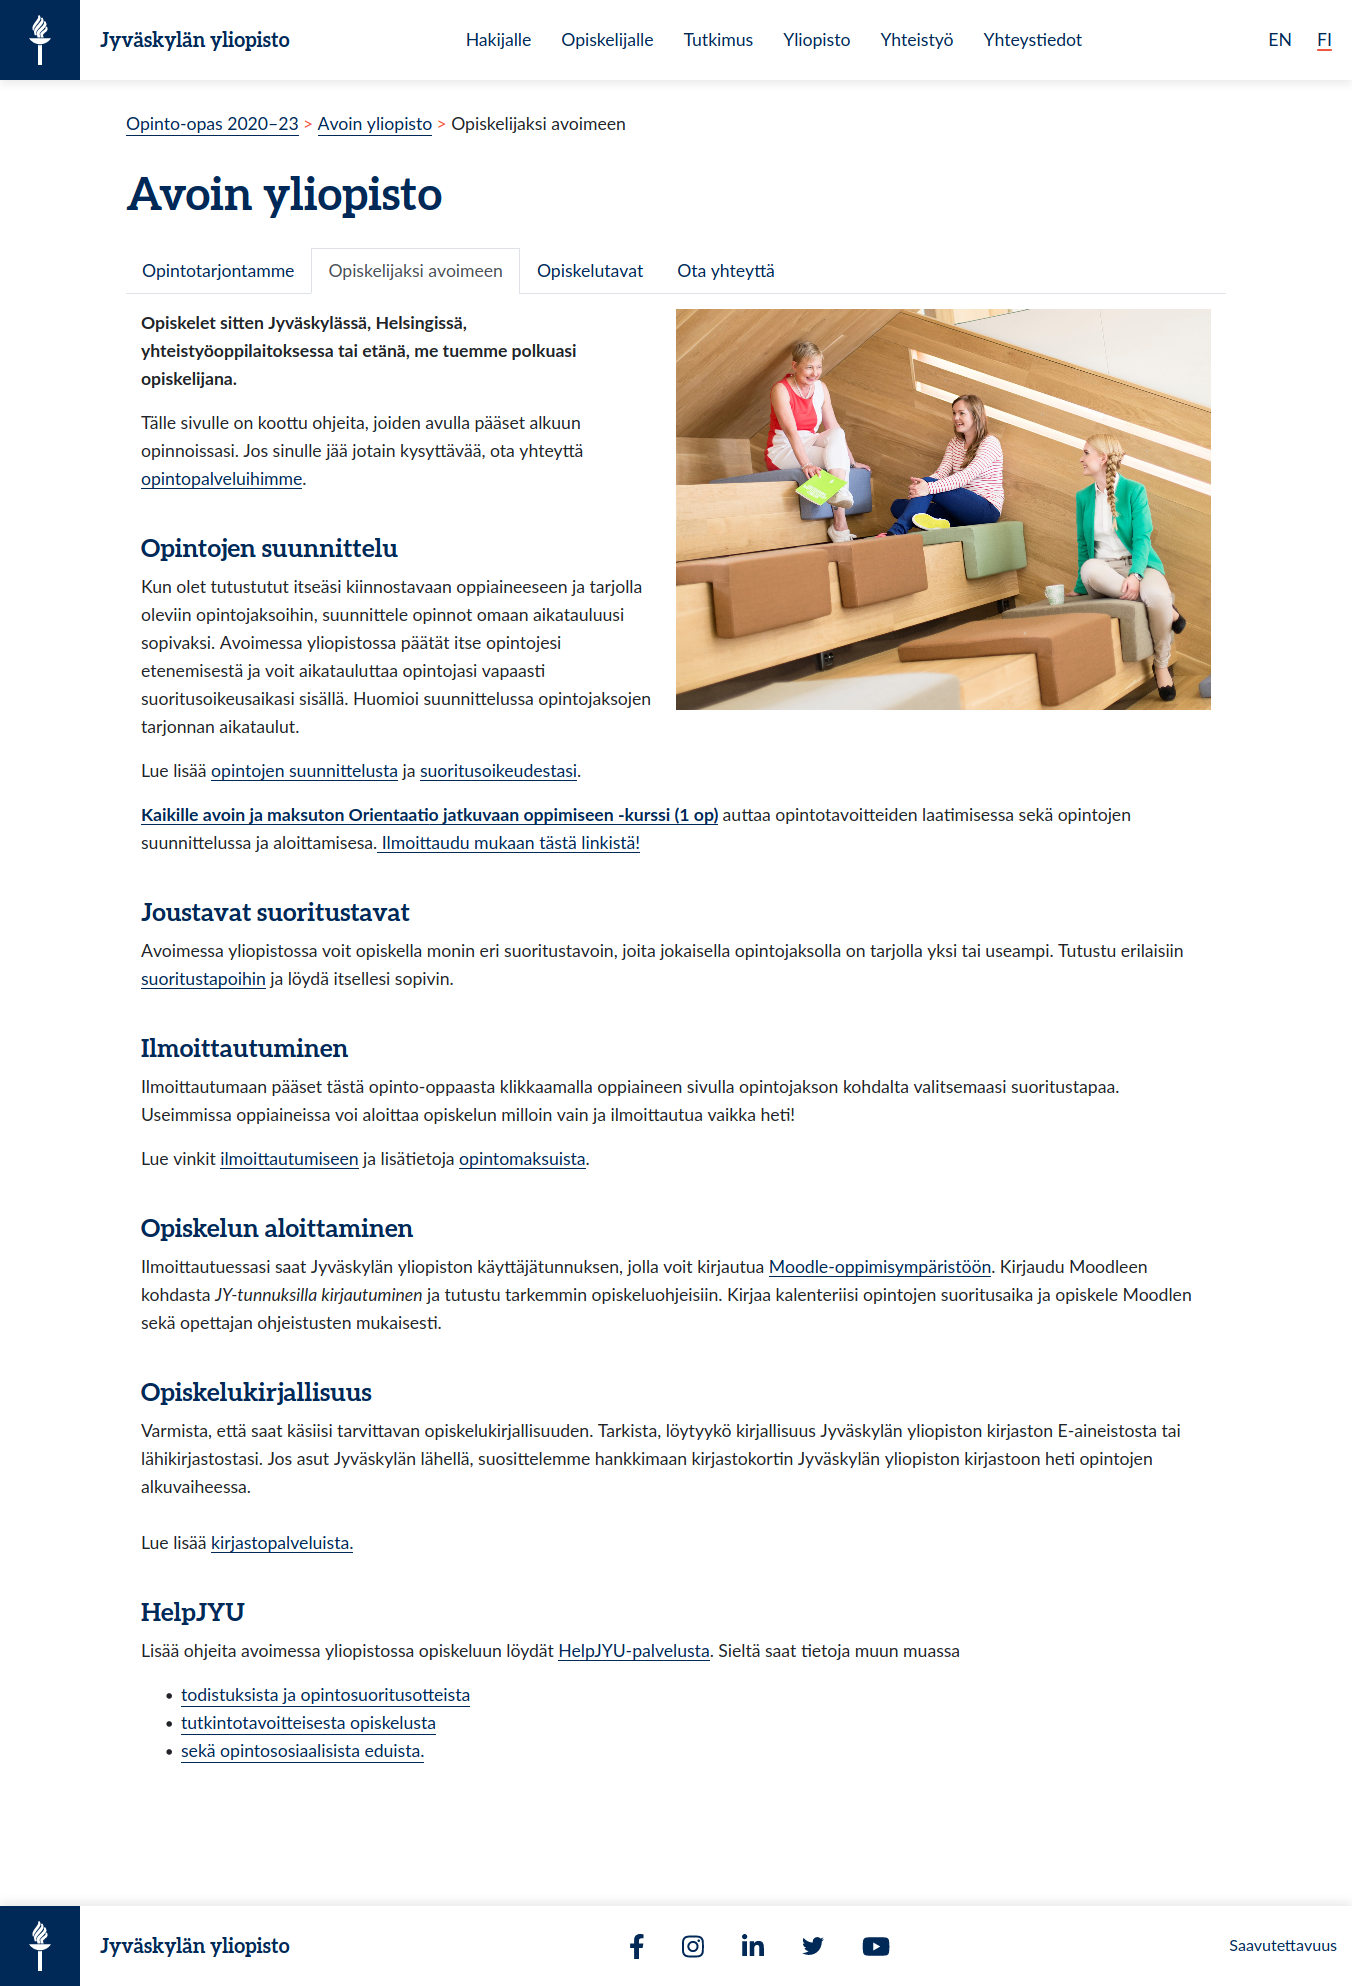
\includegraphics[width=1\paperwidth]{images/study-guide-01.png}
\end{picture}
\end{frame}

%\setbeamertemplate{background canvas}[default]
%\begin{frame}{Study Guide for University of Jyväskylä Open University}
%\begin{picture}(0,0)(29,384)
%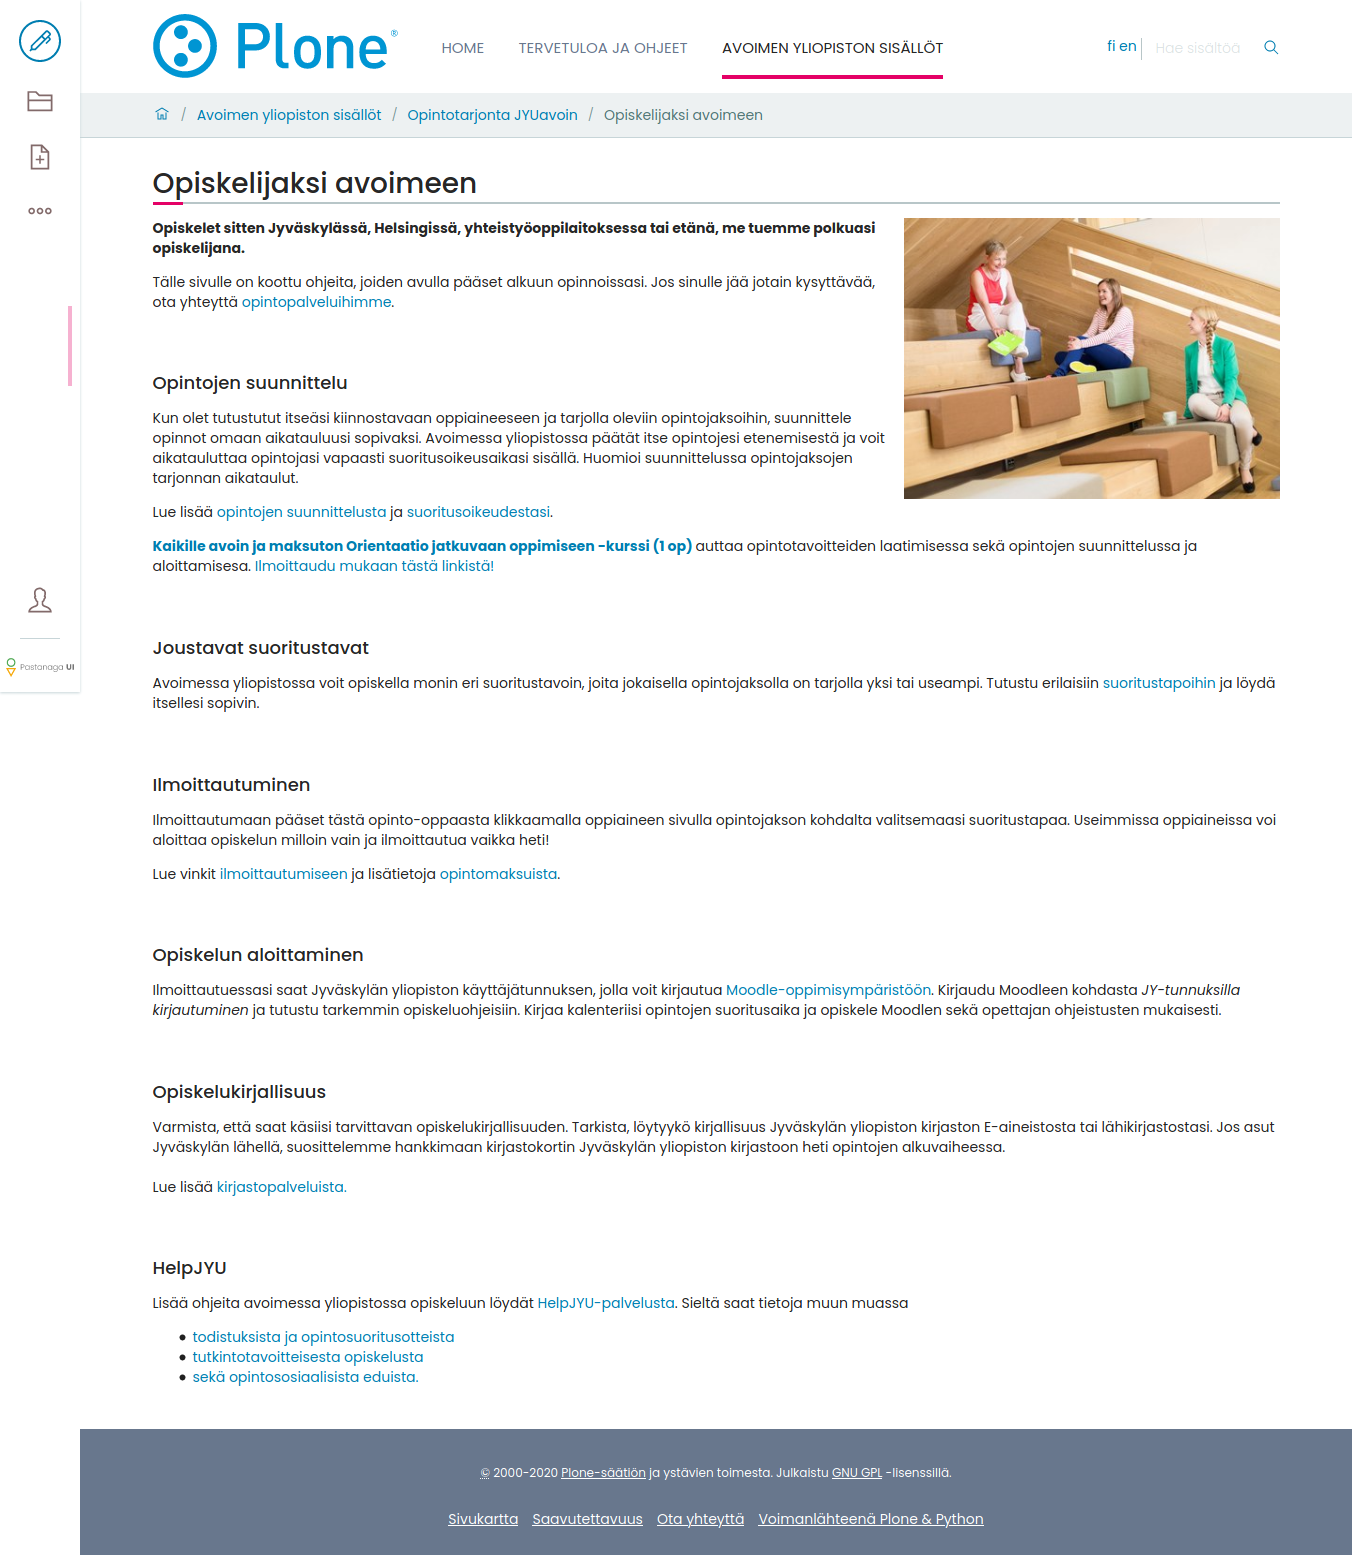
\includegraphics[width=1\paperwidth]{images/study-guide-02.png}
%\end{picture}
%\end{frame}

%---------------------------------------------------------------------------------------

\setmytemplate
\begin{frame}{Author}
  \textbf{Asko Soukka}
  \begin{itemize}
  \item[] Software architect at University of Jyväskylä Digital Services
  \end{itemize}
  \textbf{Background}
  \begin{itemize}
    \item Python developer since 2002
    \item Plone developer since 2004
    \item Full-time professional since 2008
    \item GatsbyJS user since 2018
  \end{itemize}
\end{frame}

%---------------------------------------------------------------------------------------

\setbeamertemplate{background canvas}[default]
\section{In the beginning\textellipsis}

%---------------------------------------------------------------------------------------

\setmytemplate
\begin{frame}{SISU}
  \textbf{One course management system to rule them all, but...}
  \begin{itemize}
    \item every organisation shall do their own integrations
    \item using granular REST API with deep JSON responses
  \end{itemize}
  \textbf{\href{https://studyguide.jyu.fi/}{Branded study guide DIY}}
  \begin{itemize}
    \item data in tables with JSONB column per endpoint
    \item custom API with database views and Hasura
    \item crafted with GatsbyJS + GraphQL source plugin
  \end{itemize}
\end{frame}

%---------------------------------------------------------------------------------------


\setbeamertemplate{background canvas}[default]
\section{Let there be CMS}

%---------------------------------------------------------------------------------------

\setmytemplate
\begin{frame}{Study Guide for University of Jyväskylä Open University}
  \textbf{Starting points}
  \begin{itemize}
    \item 3rd party course management system
    \item limited content authoring options
  \end{itemize}
  \textbf{Requirements}
  \begin{itemize}
    \item rich content authoring options
    \item hierarchical permission management
    \item merge structural data with custom content
    \item fast and responsive end-user experience
  \end{itemize}
\end{frame}

%---------------------------------------------------------------------------------------

\setmytemplate
\begin{frame}{Study Guide for University of Jyväskylä Open University}
  \textbf{Solution}
  \begin{itemize}
    \item[] \href{https://www.avoin.jyu.fi/opinto-opas/fi/avoinyo/}{https://www.avoin.jyu.fi/opinto-opas/fi/avoinyo/}
  \end{itemize}
  \textbf{Ingredients}
  \begin{itemize}
    \item Plone 5.2
    \item Volto
    \item GatsbyJS
  \end{itemize}
\end{frame}

%---------------------------------------------------------------------------------------

\setbeamertemplate{background canvas}[default]
\begin{frame}{Plone: No-Code Content-Type Customizations}
\begin{picture}(0,0)(29,127)
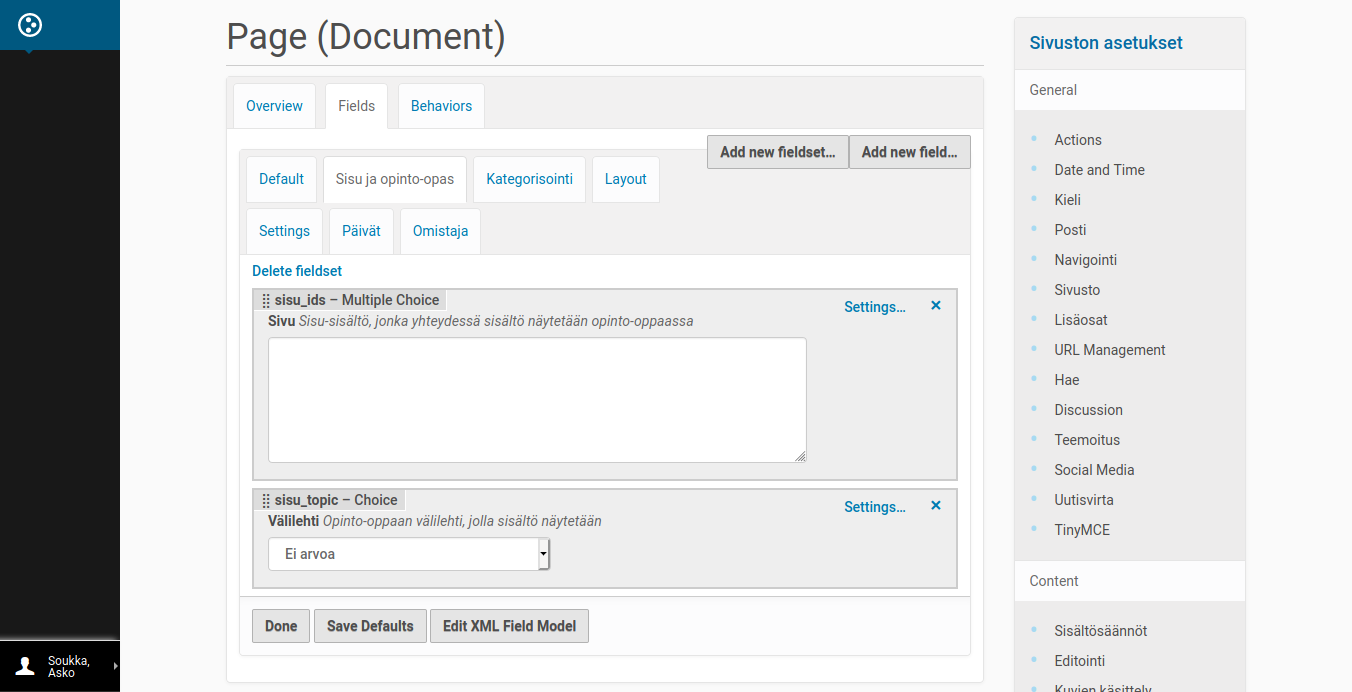
\includegraphics[width=1\paperwidth]{images/study-guide-dexterity.png}
\end{picture}
\end{frame}

\setbeamertemplate{background canvas}[default]
\begin{frame}{Volto: Auto-Complete Widgets with Custom Vocabularies}
\begin{picture}(0,0)(29,127)
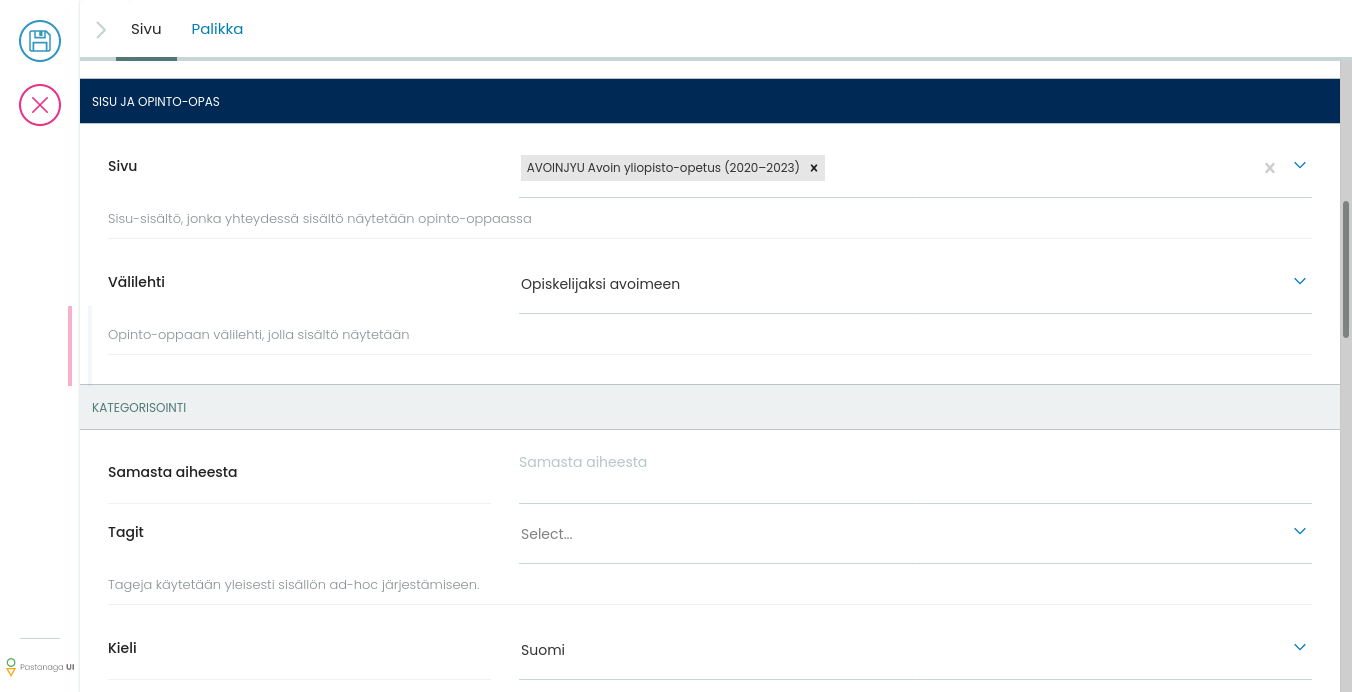
\includegraphics[width=1\paperwidth]{images/study-guide-volto.png}
\end{picture}
\end{frame}

%---------------------------------------------------------------------------------------

\setmytemplate
\begin{frame}[fragile]{GatsbyJS: Query Connected Pages with GraphQL}
\footnotesize
\begin{minted}{js}
{
  ...
  pages: allPloneDocument(filter: {
    sisu_ids: { in: [$id] },
    sisu_topic: { token: { eq: "avoin-subject" } }
  }) {
    edges {
      node {
        ...VoltoDocument
      }
    }
  }
  ...
}

\end{minted}
\end{frame}

%---------------------------------------------------------------------------------------

\setmytemplate
\begin{frame}[fragile]{ReactJS: Render Volto Layouts with React Components}
\footnotesize
\begin{minted}{js}
import VoltoDocument from '../components/VoltoDocument';

...
{props.data.pages.edges.map(({ node }) => (
  <VoltoDocument key={node.id} data={node} />
))}
...
\end{minted}
\end{frame}

%---------------------------------------------------------------------------------------

\setbeamertemplate{background canvas}[default]
\section{GatsbyJS Recap}

%---------------------------------------------------------------------------------------

\setmytemplate
\begin{frame}{JavaScript, API \& Markup}
  GatsbyJS is a ReactJS-based site generator\par
  \vspace{12pt}\par
  \textbf{Why GatsbyJS?}
  \begin{itemize}
    \item multi-source plugin architecture
    \item GraphQL based data lookup
    \item convention over configuration
    \item seamless developer experience
    \item comprehensive documentation
  \end{itemize}
\end{frame}

%---------------------------------------------------------------------------------------

\setbeamertemplate{background canvas}[default]
\section{gatsby-source-plone}

%---------------------------------------------------------------------------------------

\setmytemplate
\begin{frame}{gatsby-source-plone}
  \href{https://github.com/collective/gatsby-source-plone/}{https://github.com/collective/gatsby-source-plone/}\par
  \vspace{12pt}\par
  \textbf{Features}
  \begin{itemize}
    \item supports default types and most TTW types
    \item supports files and images from default types
    \item supports richtext from default types
    \item resolves linked objects from default types
    \item incremental updates by modification date
  \end{itemize}
\end{frame}

%---------------------------------------------------------------------------------------

\setmytemplate
\begin{frame}[fragile]{Basic configuration}
\footnotesize
\begin{minted}{js}
{
  resolve: 'gatsby-source-plone',
  options: {
    baseUrl: 'https://plonedemo.kitconcept.com/en',
  },
},
{
  resolve: 'gatsby-source-filesystem',
  options: {
    path: `${__dirname}/src/static`,
  },
},
\end{minted}
\end{frame}

\setmytemplate
\begin{frame}[fragile]{Advanced configuration}
\footnotesize
\begin{minted}{js}
{
  resolve: 'gatsby-source-plone',
  options: {
    baseUrl: 'https://plonedemo.kitconcept.com',
    searchParams: {
      path: [
        '/en/'
      ],
    },
    token: process.env.PLONE_TOKEN,
  },
},
\end{minted}
\end{frame}

\setbeamertemplate{background canvas}[default]
\begin{frame}{iGraphQL}
\begin{picture}(0,0)(29,149)
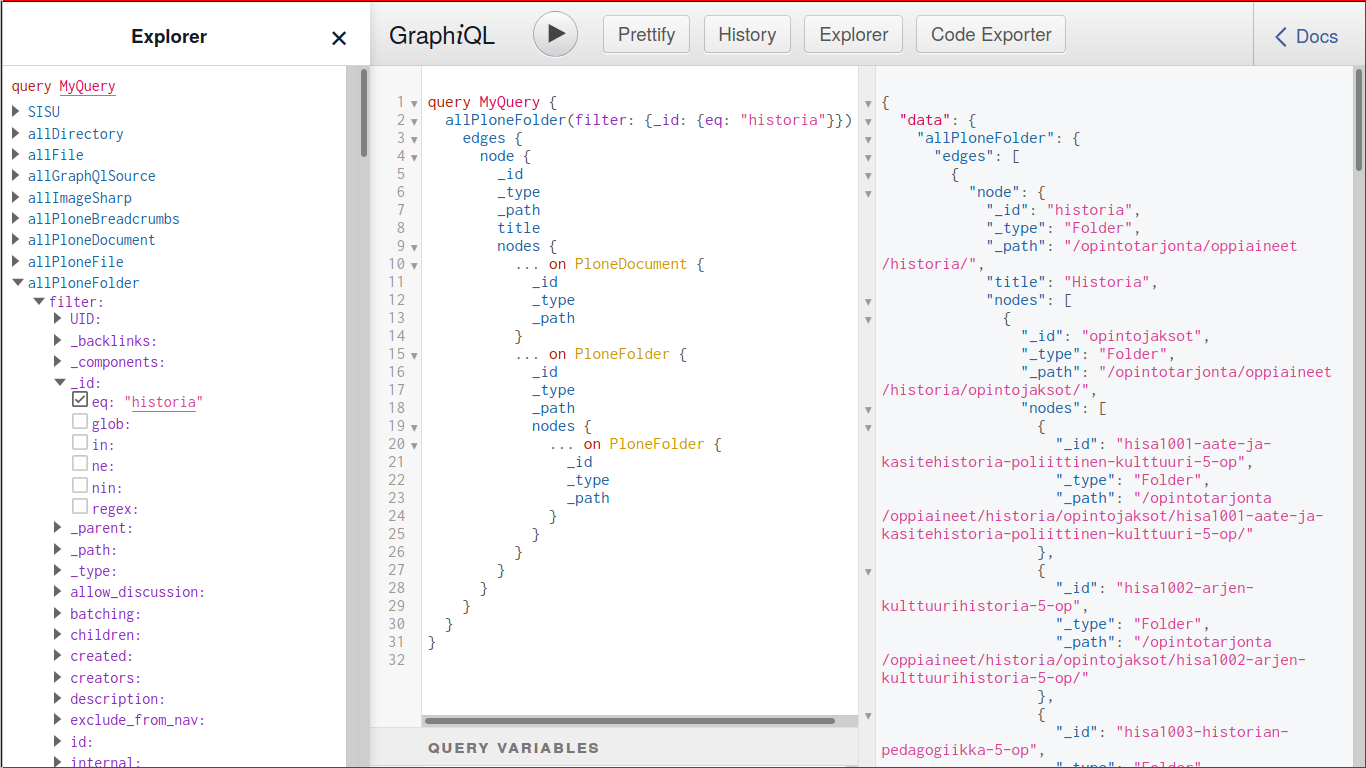
\includegraphics[trim={0 0 1pt 1pt},clip,width=1\paperwidth]{images/gatsby-source-plone-igraphql.png}
\end{picture}
\end{frame}

%---------------------------------------------------------------------------------------

\setmytemplate
\begin{frame}{Not Only Rainbows and Unicorns}
  \textbf{Full “GatsbyJS experience” requires practice}
  \begin{itemize}
    \item query connected pages, images and files
    \item replace inline links with GatsbyJS links
    \item replace inline images with GatsbyJS images
    \item replace file links with direct download
  \end{itemize}
  \textbf{Using @plone/volto seemed like a good idea\ldots}
  \begin{itemize}
    \item required Webpack overrides to be importable
    \item could not be used for images and links
  \end{itemize}
\end{frame}

%---------------------------------------------------------------------------------------

\setbeamertemplate{background canvas}[default]
\section{Discussion}

%---------------------------------------------------------------------------------------

\setmytemplate
\begin{frame}{Discussion}
  \textbf{GatsbyJS – the ugly parts}
  \begin{itemize}
    \item GraphQL source plugin cannot cache
    \item build may take hours
    \item build may take gigabytes of memory
    \item build result is readonly
    \item monorepo is painful to follow
  \end{itemize}
\end{frame}

%---------------------------------------------------------------------------------------

\setbeamertemplate{background canvas}[default]
\begin{frame}[standout]
\vfill

\includegraphics[height=0.50\paperheight]{images/plone-icon-hearts.png}
\par
\href{https://datakurre.github.io/ploneconf2020/}{datakurre.github.io/ploneconf2020}
\end{frame}

%---------------------------------------------------------------------------------------

\end{document}
